\clearpage
\section*{三、结果与分析}

\subsection*{1. 力敏传感器定标}

我以砝码重力 $F$ 为纵坐标、平均读数 $U$ 为横坐标，对 8 组数据作最小二乘拟合 $F=KU+b$，结果见图（a）：

\[
K=4.2569\times10^{-5}\ \mathrm{N/mV},\qquad b=-4.4\times10^{-5}\ \mathrm{N},\qquad r=0.999998.
\]

斜率的标准差为 $s_K=3.68\times10^{-8}\ \mathrm{N/mV}$。按课件要求，以 3 倍标准差估计 $K$ 的不确定度，即 $u(K)=3s_K=1.10\times10^{-7}\ \mathrm{N/mV}$，故

\[
K=(4.257\pm0.011)\times10^{-5}\ \mathrm{N/mV}.
\]

\begin{figure}[H]\centering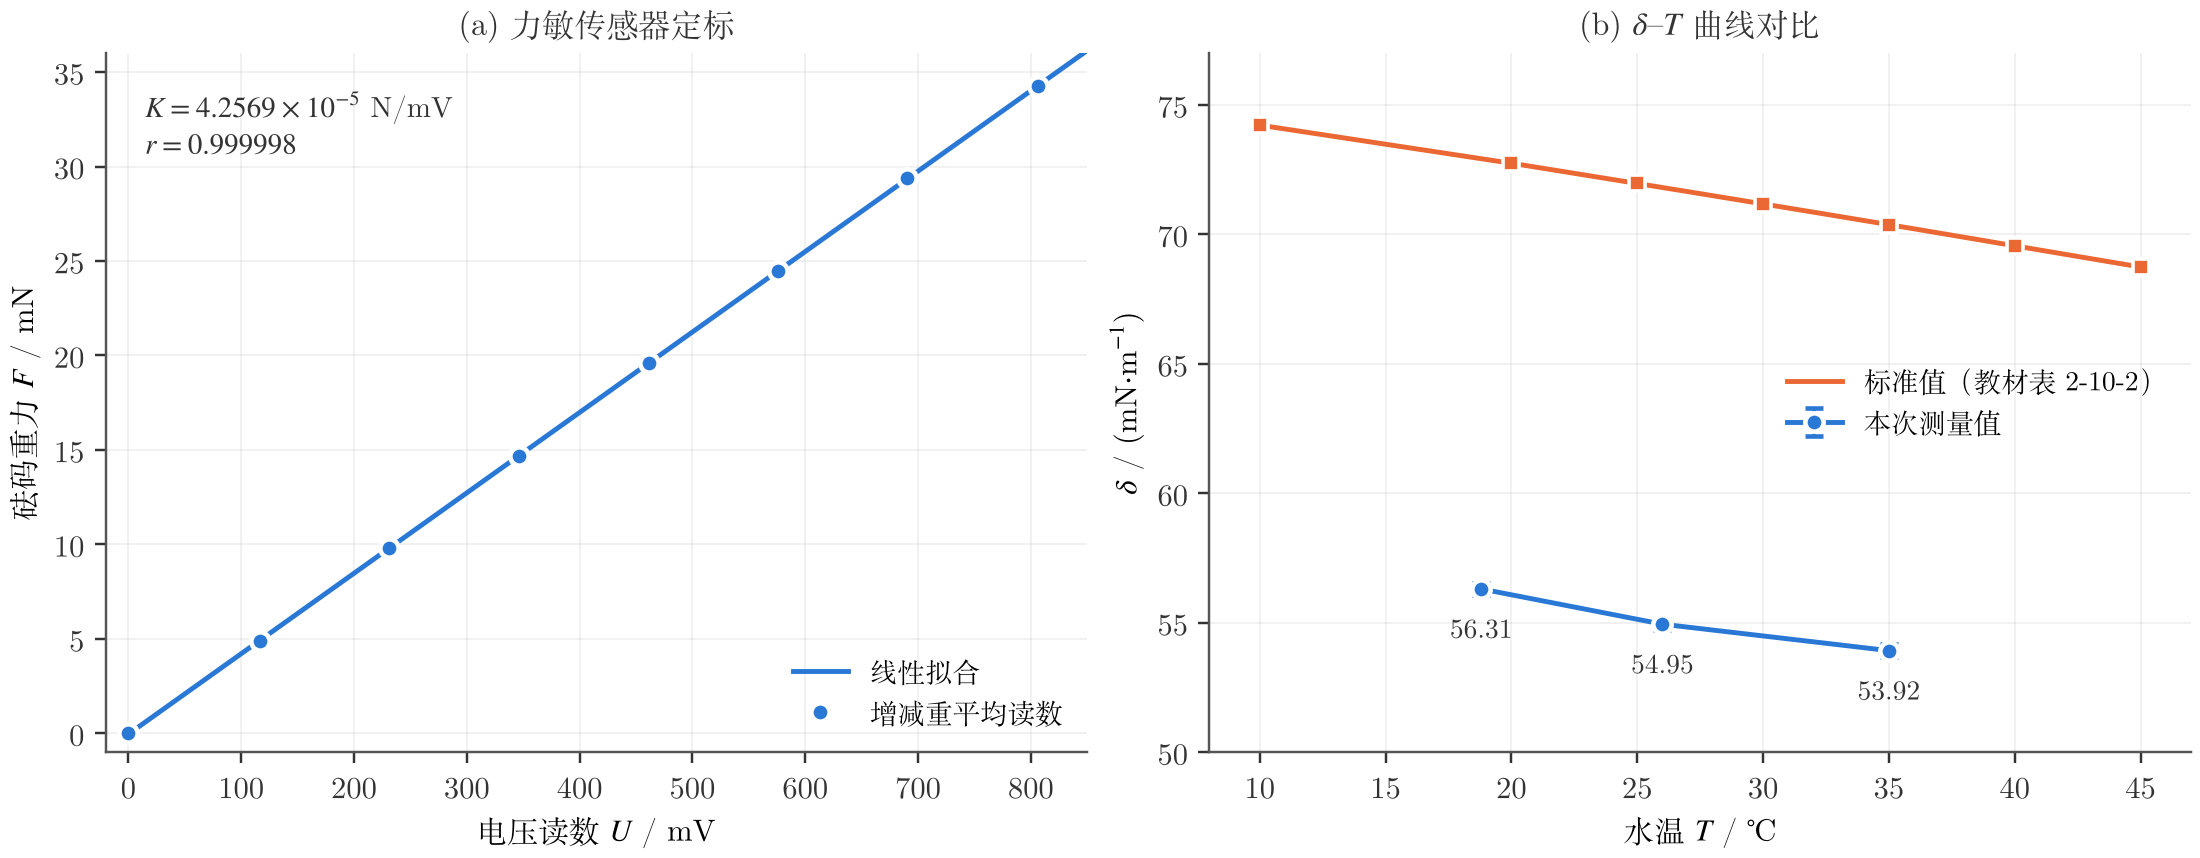
\includegraphics[width=\linewidth]{../assets/surface_tension.png}\caption{力敏传感器定标拟合与 $\delta$–$T$ 曲线对比}\end{figure}

\subsection*{2. 圆环内外径}

两组直径各测 6 次，A 类标准不确定度取 $u_A=s/\sqrt6$。游标卡尺的允许误差限为 $\Delta=0.02\,\mathrm{mm}$，按均匀分布得 B 类分量

\[
u_B=\frac{\Delta}{\sqrt3}=\frac{0.02}{\sqrt3}\,\mathrm{mm}=0.012\,\mathrm{mm}.
\]

\begin{center}\small
\begin{tabular}{cccccc}
\toprule
量 & 平均值/mm & $s$/mm & $u_A$/mm & $u_B$/mm & $u=\sqrt{u_A^2+u_B^2}$/mm \\
\midrule
内径 $d_1$ & 32.760 & 0.058 & 0.024 & 0.012 & 0.026 \\
外径 $d_2$ & 34.890 & 0.033 & 0.013 & 0.012 & 0.018 \\
\bottomrule\end{tabular}\end{center}

因此 $d_1=(32.760\pm0.026)\,\mathrm{mm}$，$d_2=(34.890\pm0.018)\,\mathrm{mm}$，$d_1+d_2=67.650\,\mathrm{mm}$。

\subsection*{3. 表面张力系数及其不确定度}

每个温度下的 $\Delta U$ 取 6 次平均，A 类分量为 $u_A=s/\sqrt6$。课堂给出的电压允差为 $0.1\,\mathrm{mV}$，而 $\Delta U$ 是 $U_{\max}$ 与 $U_{\text{环}}$ 两次读数之差，按均匀分布得

\[
u_B(\Delta U)=\sqrt2\times\frac{0.1}{\sqrt3}\,\mathrm{mV}=0.082\,\mathrm{mV}.
\]

再由 $\delta=\dfrac{K\Delta U}{\pi(d_1+d_2)}$ 计算表面张力系数，并按课堂给出的传播律合成

\[
\frac{u(\delta)}{\delta}=\sqrt{\left(\frac{u(K)}{K}\right)^{2}+\left(\frac{u(\Delta U)}{\Delta U}\right)^{2}+\left(\frac{u(d_1)}{d_1+d_2}\right)^{2}+\left(\frac{u(d_2)}{d_1+d_2}\right)^{2}}.
\]

以室温为例，$\overline{\Delta U}=1686.7/6\,\mathrm{mV}=281.117\,\mathrm{mV}$，则

\[
\delta=\frac{4.2569\times10^{-5}\times281.117}{\pi\times0.067650}\ \mathrm{N/m}=5.6308\times10^{-2}\ \mathrm{N/m}.
\]

四项相对不确定度依次为 $0.260\%$、$0.340\%$、$0.039\%$ 和 $0.026\%$，合成后 $u(\delta)/\delta=0.43\%$。三个温度的计算结果如下。

\begin{center}\small
\begin{tabular}{ccccccc}
\toprule
水温 & $\overline{\Delta U}$/mV & $s$/mV & $u_A$/mV & $u(\Delta U)$/mV & $\delta$/(mN$\cdot$m$^{-1}$) & $u(\delta)$/(mN$\cdot$m$^{-1}$) \\
\midrule
$18.8\,{}^\circ\mathrm{C}$ & 281.12 & 2.33 & 0.95 & 0.96 & 56.31 & 0.24 \\
$26\,{}^\circ\mathrm{C}$ & 274.32 & 1.99 & 0.81 & 0.82 & 54.95 & 0.22 \\
$35\,{}^\circ\mathrm{C}$ & 269.22 & 2.33 & 0.95 & 0.96 & 53.92 & 0.24 \\
\bottomrule\end{tabular}\end{center}

因此本次测量结果为

\[
\delta_{18.8\,{}^\circ\mathrm{C}}=(56.31\pm0.24)\times10^{-3}\ \mathrm{N/m},
\]

\[
\delta_{26\,{}^\circ\mathrm{C}}=(54.95\pm0.22)\times10^{-3}\ \mathrm{N/m},
\]

\[
\delta_{35\,{}^\circ\mathrm{C}}=(53.92\pm0.24)\times10^{-3}\ \mathrm{N/m}.
\]

\subsection*{4. 与标准值比较}

标准值由教材表 2-10-2 线性插值得到，相对误差 $E=(\delta-\delta_0)/\delta_0\times100\%$。

\begin{center}\small
\begin{tabular}{cccc}
\toprule
水温 & 测量值 $\delta$/(mN$\cdot$m$^{-1}$) & 标准值 $\delta_0$/(mN$\cdot$m$^{-1}$) & 相对误差 $E$ \\
\midrule
$18.8\,{}^\circ\mathrm{C}$ & 56.31 & 72.93 & −22.8\% \\
$26\,{}^\circ\mathrm{C}$ & 54.95 & 71.81 & −23.5\% \\
$35\,{}^\circ\mathrm{C}$ & 53.92 & 70.38 & −23.4\% \\
\bottomrule\end{tabular}\end{center}

由图（b）可见，测得的 $\delta$ 随温度升高而减小，在 $18.8\sim35\,{}^\circ\mathrm{C}$ 内平均每升高 $1\,{}^\circ\mathrm{C}$ 下降约 $0.146\,\mathrm{mN/m}$，与标准值的 $0.157\,\mathrm{mN/m}$ 接近。不过，三组结果整体比标准值低约 23\%，而合成不确定度只有约 0.4\%。因此，偏差主要来自不确定度未能覆盖的系统误差，而不是读数的随机波动。

\subsection*{5. 误差分析}

\begin{enumerate}
\item \textbf{水不纯净。} 实验用水并非纯水，器皿敞口放置时还会落入灰尘。杂质中的表面活性物质聚集在液面，使表面张力降低。三个温度的偏差都接近 23\%，也说明这是一种系统性偏低。
\item \textbf{圆环沾有油污。} 取放圆环时手会接触环面，油脂进入液面后降低了表面张力；同时环面润湿变差，接触角增大，液膜在达到最大拉力前就从环上脱开，使 $U_{\max}$ 偏小。
\item \textbf{调零时圆环带水。} 本次只在初始时调零，此后 $U_{\text{环}}$ 都记为 0，没有在每次液膜破裂后重新读基线。若调零时圆环上附着水，零点就包含了这部分水的重力，拉脱后附着水量变化，$\Delta U$ 因此被少计。
\item \textbf{仪器噪声与光标读数。} 拉力曲线上叠加有噪声。同时，示波器纵轴为 $200\,\mathrm{mV/DIV}$ 时，光标的最小步进约为 $3.1\,\mathrm{mV}$，所以同一温度下的 $\Delta U$ 只出现 277.5、280.6、283.7 mV 等相隔一格的数值。这一步进属于读数分辨力，而不是仪器允许误差限，因此 B 类分量仍按课堂给出的 0.1 mV 评定；它造成的波动已反映在 A 类分量中（$s\approx2.3\,\mathrm{mV}$）。即使把半个步进作为误差界限估算，三个温度的 $u(\delta)/\delta$ 也只从 0.40\%～0.44\% 增大到 0.52\%～0.55\%，远小于约 23\% 的偏差。若要减小这一影响，可在信号不超出屏幕的前提下改用更小的纵轴档位，或改用仪器的数字电压表读数。
\item \textbf{液面下降与震动。} 降低液面过快或桌面震动，会使液膜提前破裂，读数偏小。同一温度下 6 次 $\Delta U$ 最多相差约 6 mV，主要来自这一随机因素。

\end{enumerate}
